% SETUP
\documentclass{article}
\usepackage{geometry}
\usepackage{fancyhdr}
\usepackage{titlesec}
\usepackage{tabularx}
\usepackage[none]{hyphenat}
\usepackage{multicol}
\usepackage{hhline}
\usepackage{caption}
\usepackage{graphicx}
\usepackage{placeins}
\usepackage{biblatex}
\usepackage{amsmath}
\addbibresource{references.bib}
\geometry{
	a4paper, 
	total={170mm,257mm}, 
	left=25mm, 
	right=25mm,
	top=30mm, 
	bottom=30mm}

% FIGURES IN MULTICOLS
\newenvironment{Figure}
  {\par\medskip\noindent\minipage{\linewidth}}
  {\endminipage\par\medskip}

% SECTION TITLE FORMAT
\titleformat{\section}
  {\normalfont\bfseries}{\thesection}{1em}{}[{\titlerule[0.3pt]}]

% HEADER & FOOTER
\pagestyle{fancy}
\renewcommand{\headrulewidth}{0pt}
\chead{\large Progress Report 2: Disentanglement by Cross Training\\
Using FUNIT Implementation}
\lhead{}
\rhead{}
\cfoot{}

\begin{document}

% CONTACT
\begin{table}[!h]
\center
\begin{tabular}{|l|l|l|}
\hline
\textbf{Name}             & \textbf{Student ID} & \textbf{E-Mail}            \\ \hhline{|=|=|=|}
Li Nguyen        & 934644485  & li.nguyen@tum.de  \\ \hline
Alexander Koenig & 918254061  & awc.koenig@tum.de \\ \hline
\end{tabular}
\end{table}

\begin{figure}[h!]
	\centering 
	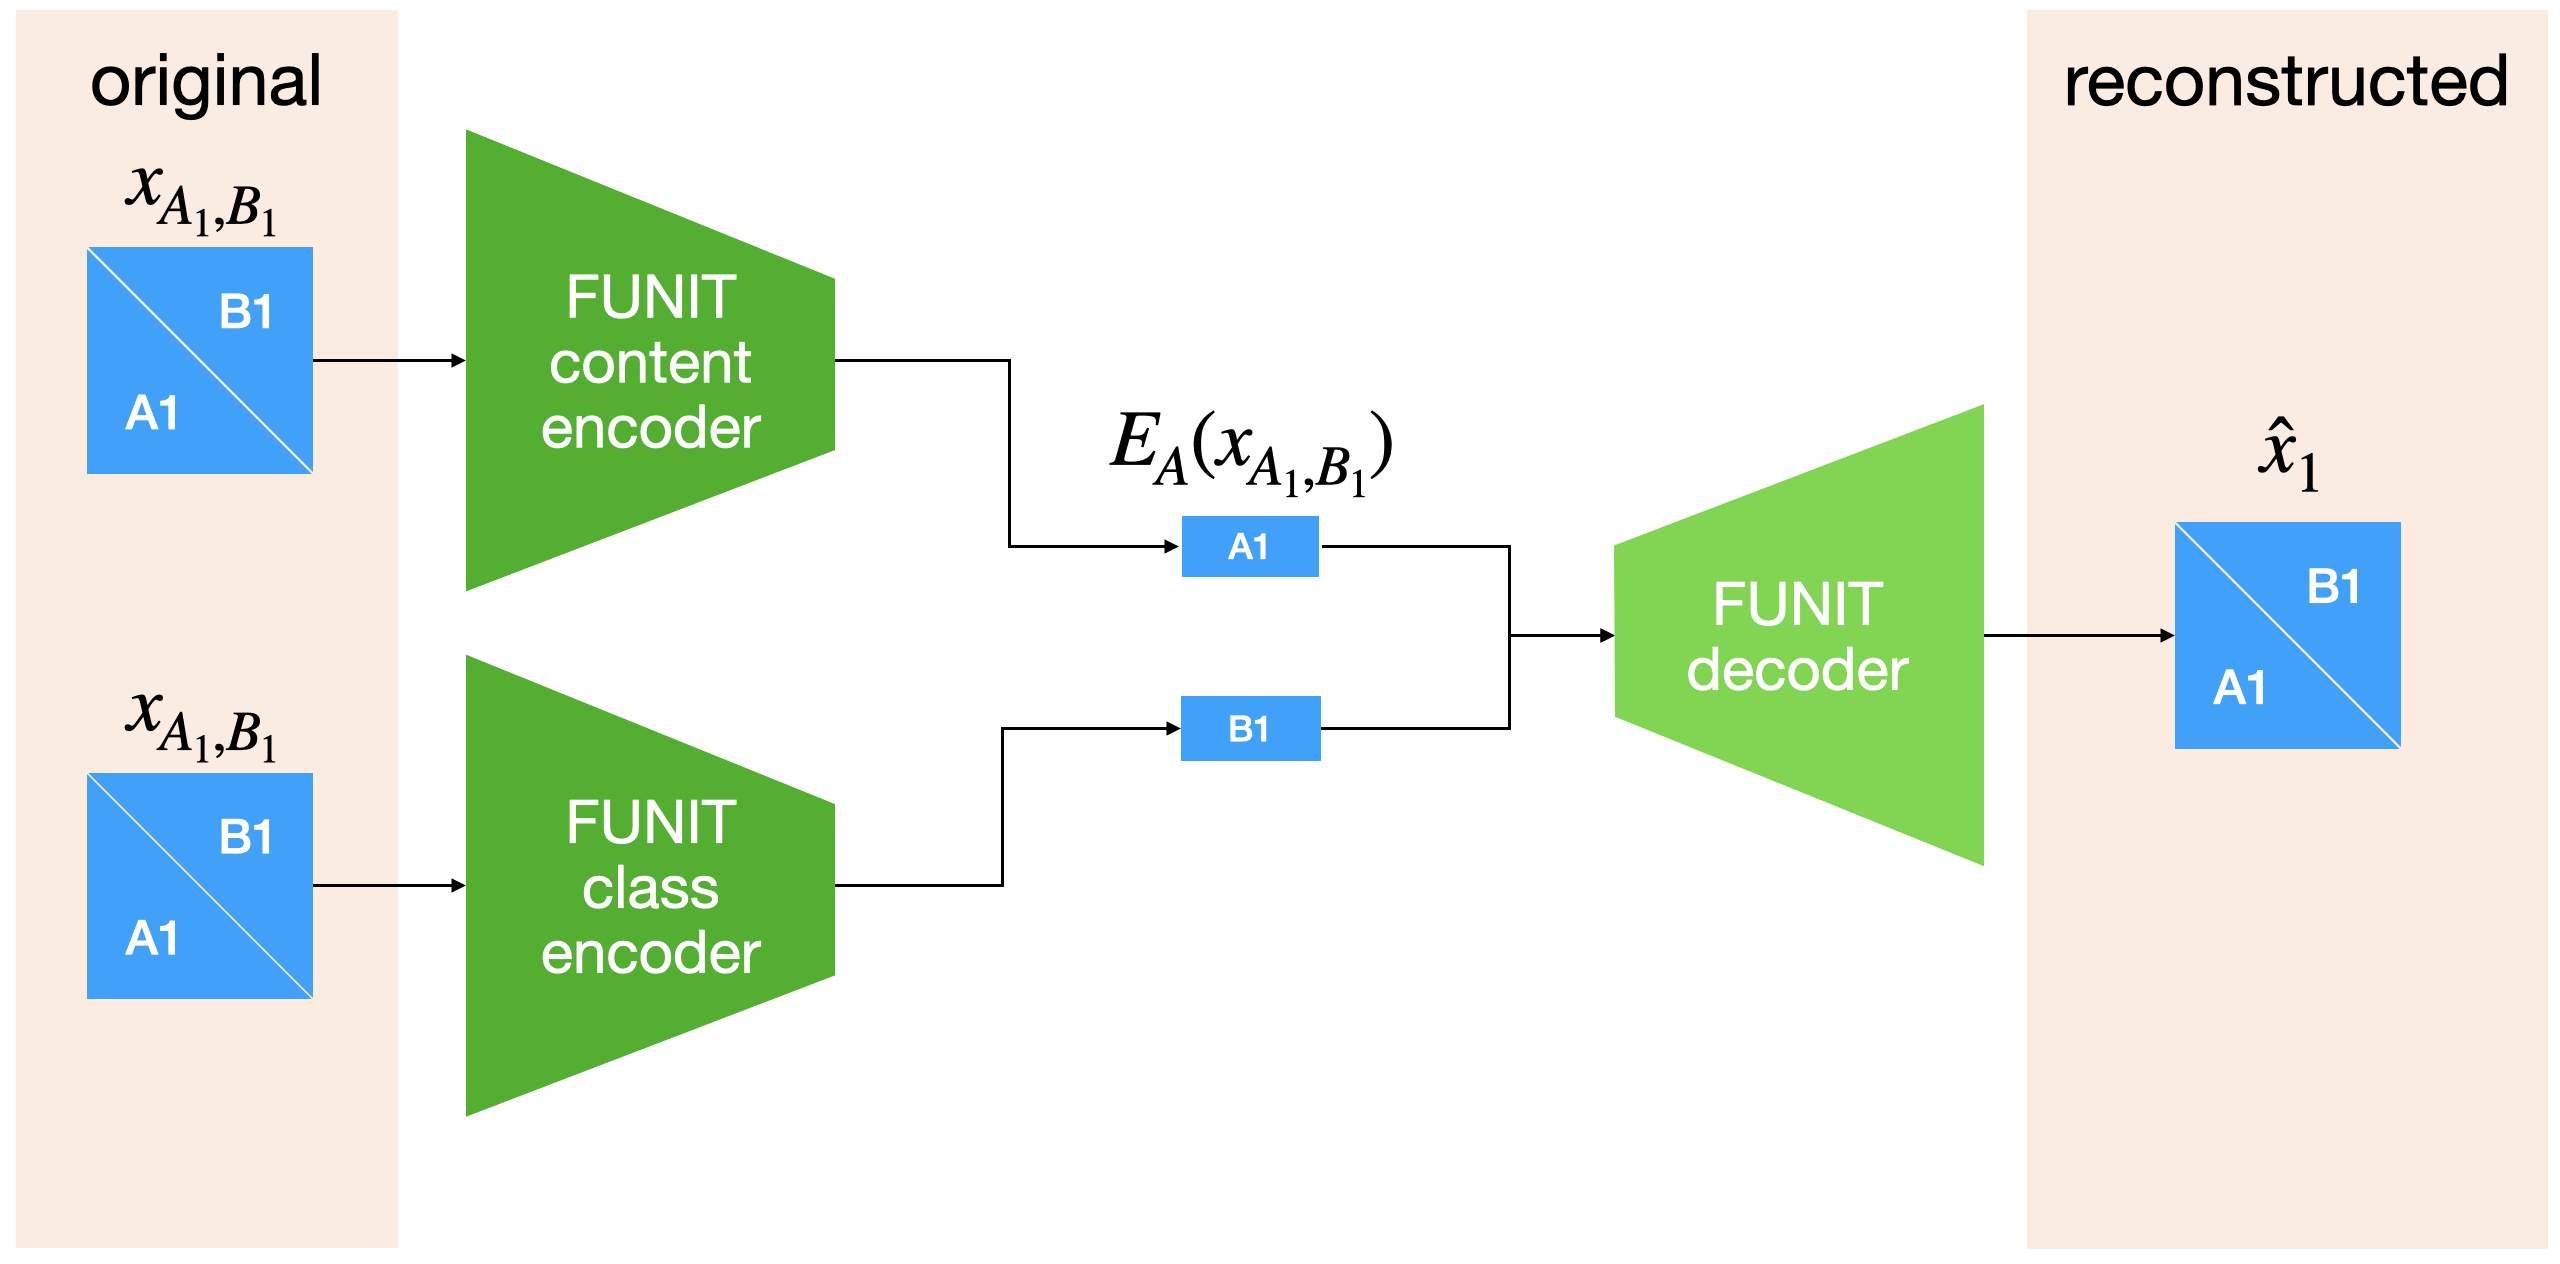
\includegraphics[width=1.0\linewidth]{figures/step1.png}
	\caption{Step 1: Simple Reconstruction using FUNIT encoder and decoder architecture and VGG perceptual loss}
	\label{fig:step1}
\end{figure}

\begin{figure}[ht]
	\centering 
	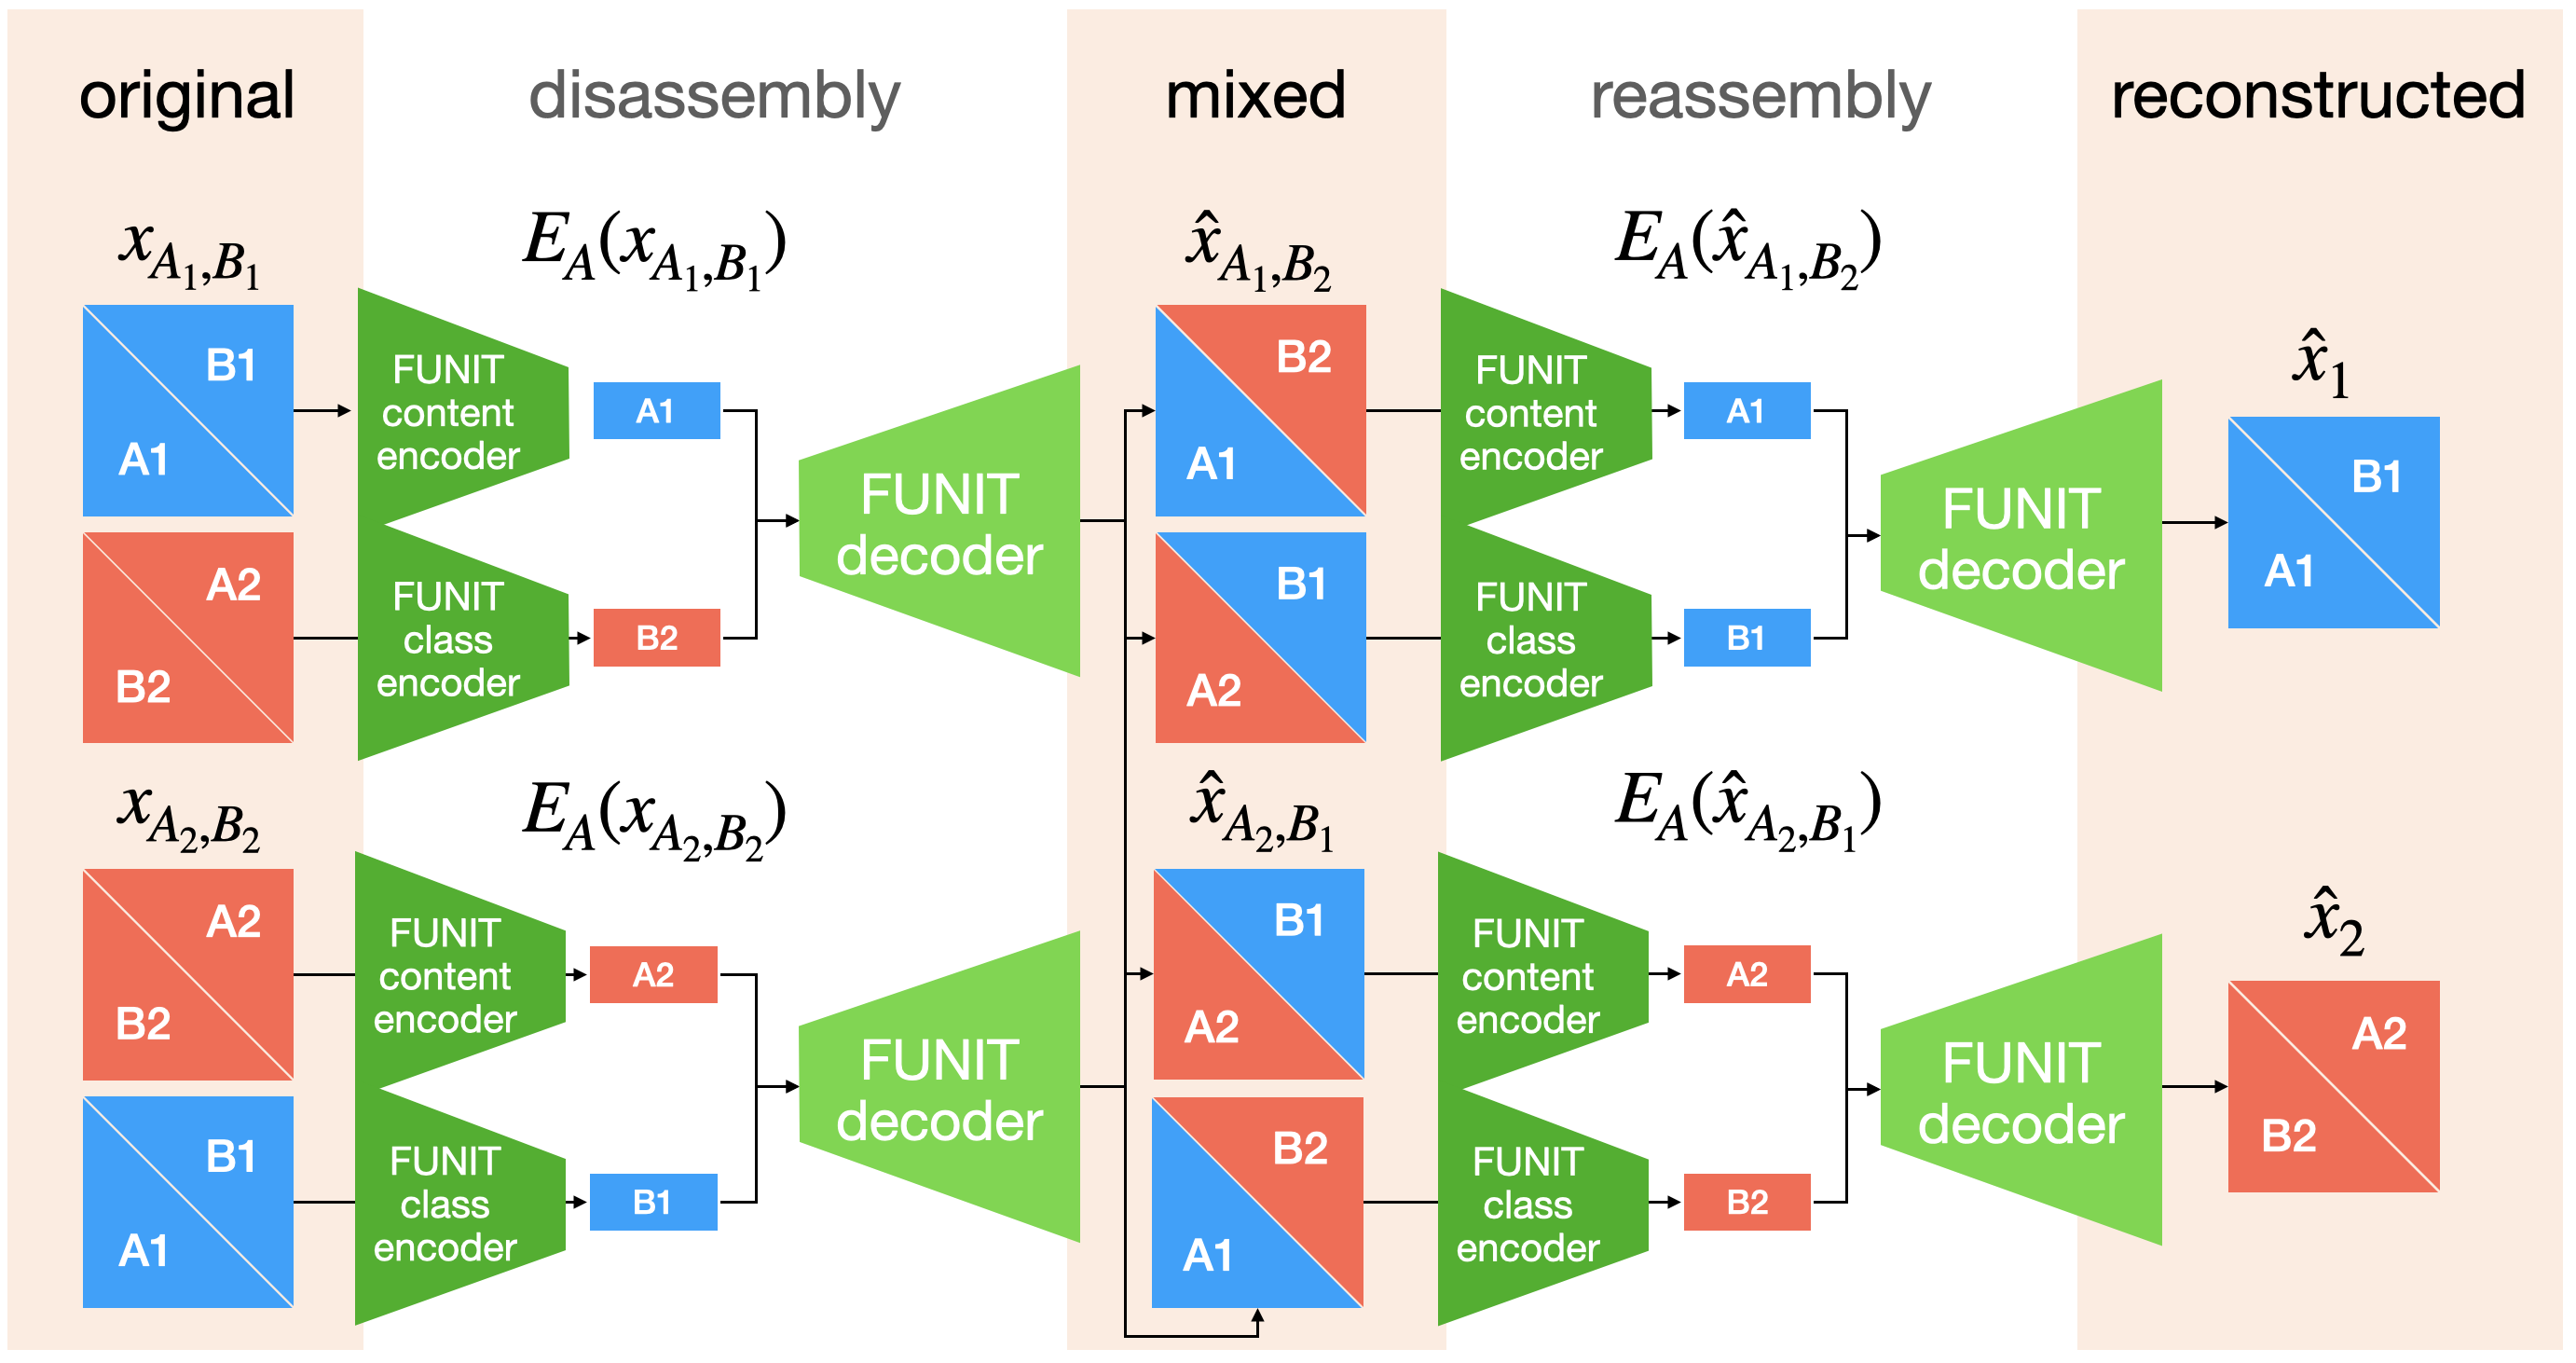
\includegraphics[width=0.95\linewidth]{figures/step2.png}
	\caption{FUNIT encoders and decoder integrated in our G2G architecture}
	\label{fig:step2}
\end{figure}

\begin{figure}[ht]
	\centering 
	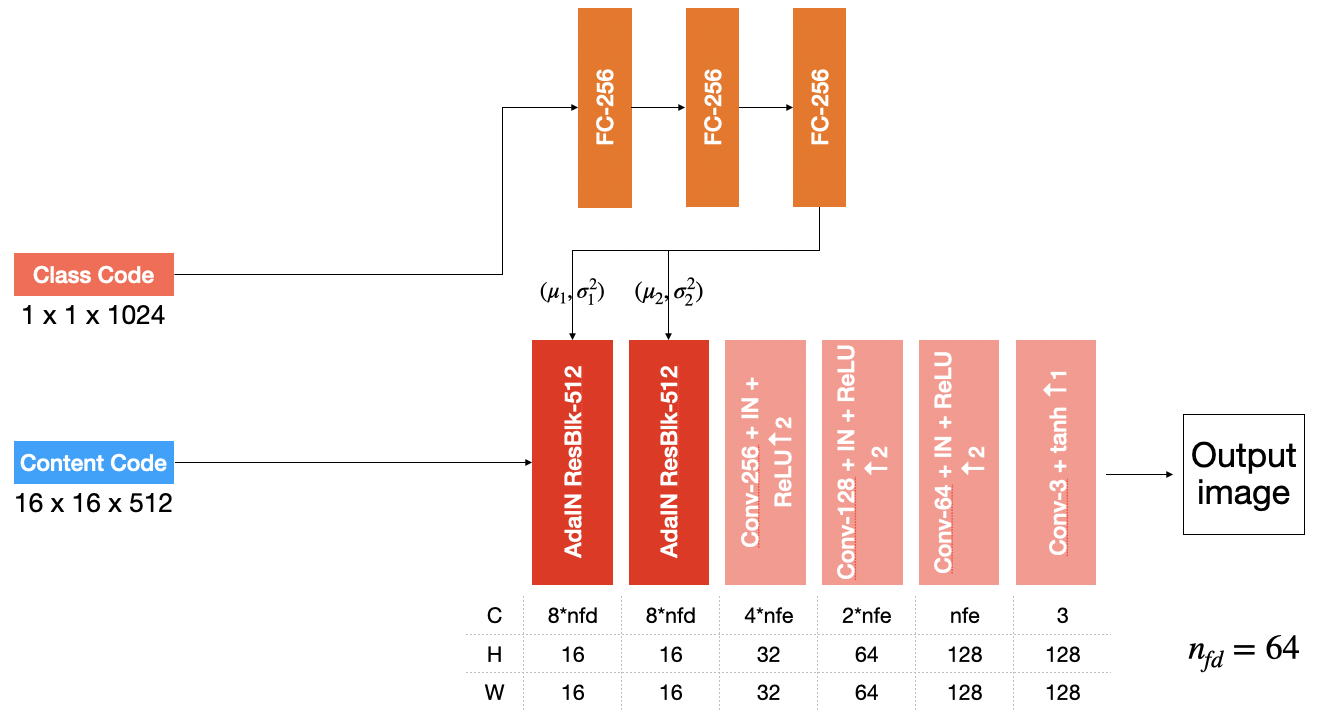
\includegraphics[width=0.95\linewidth]{figures/decoder.png}
	\caption{FUNIT decoder}
	\label{fig:decoder}
\end{figure}

\begin{figure}[ht]
	\centering 
	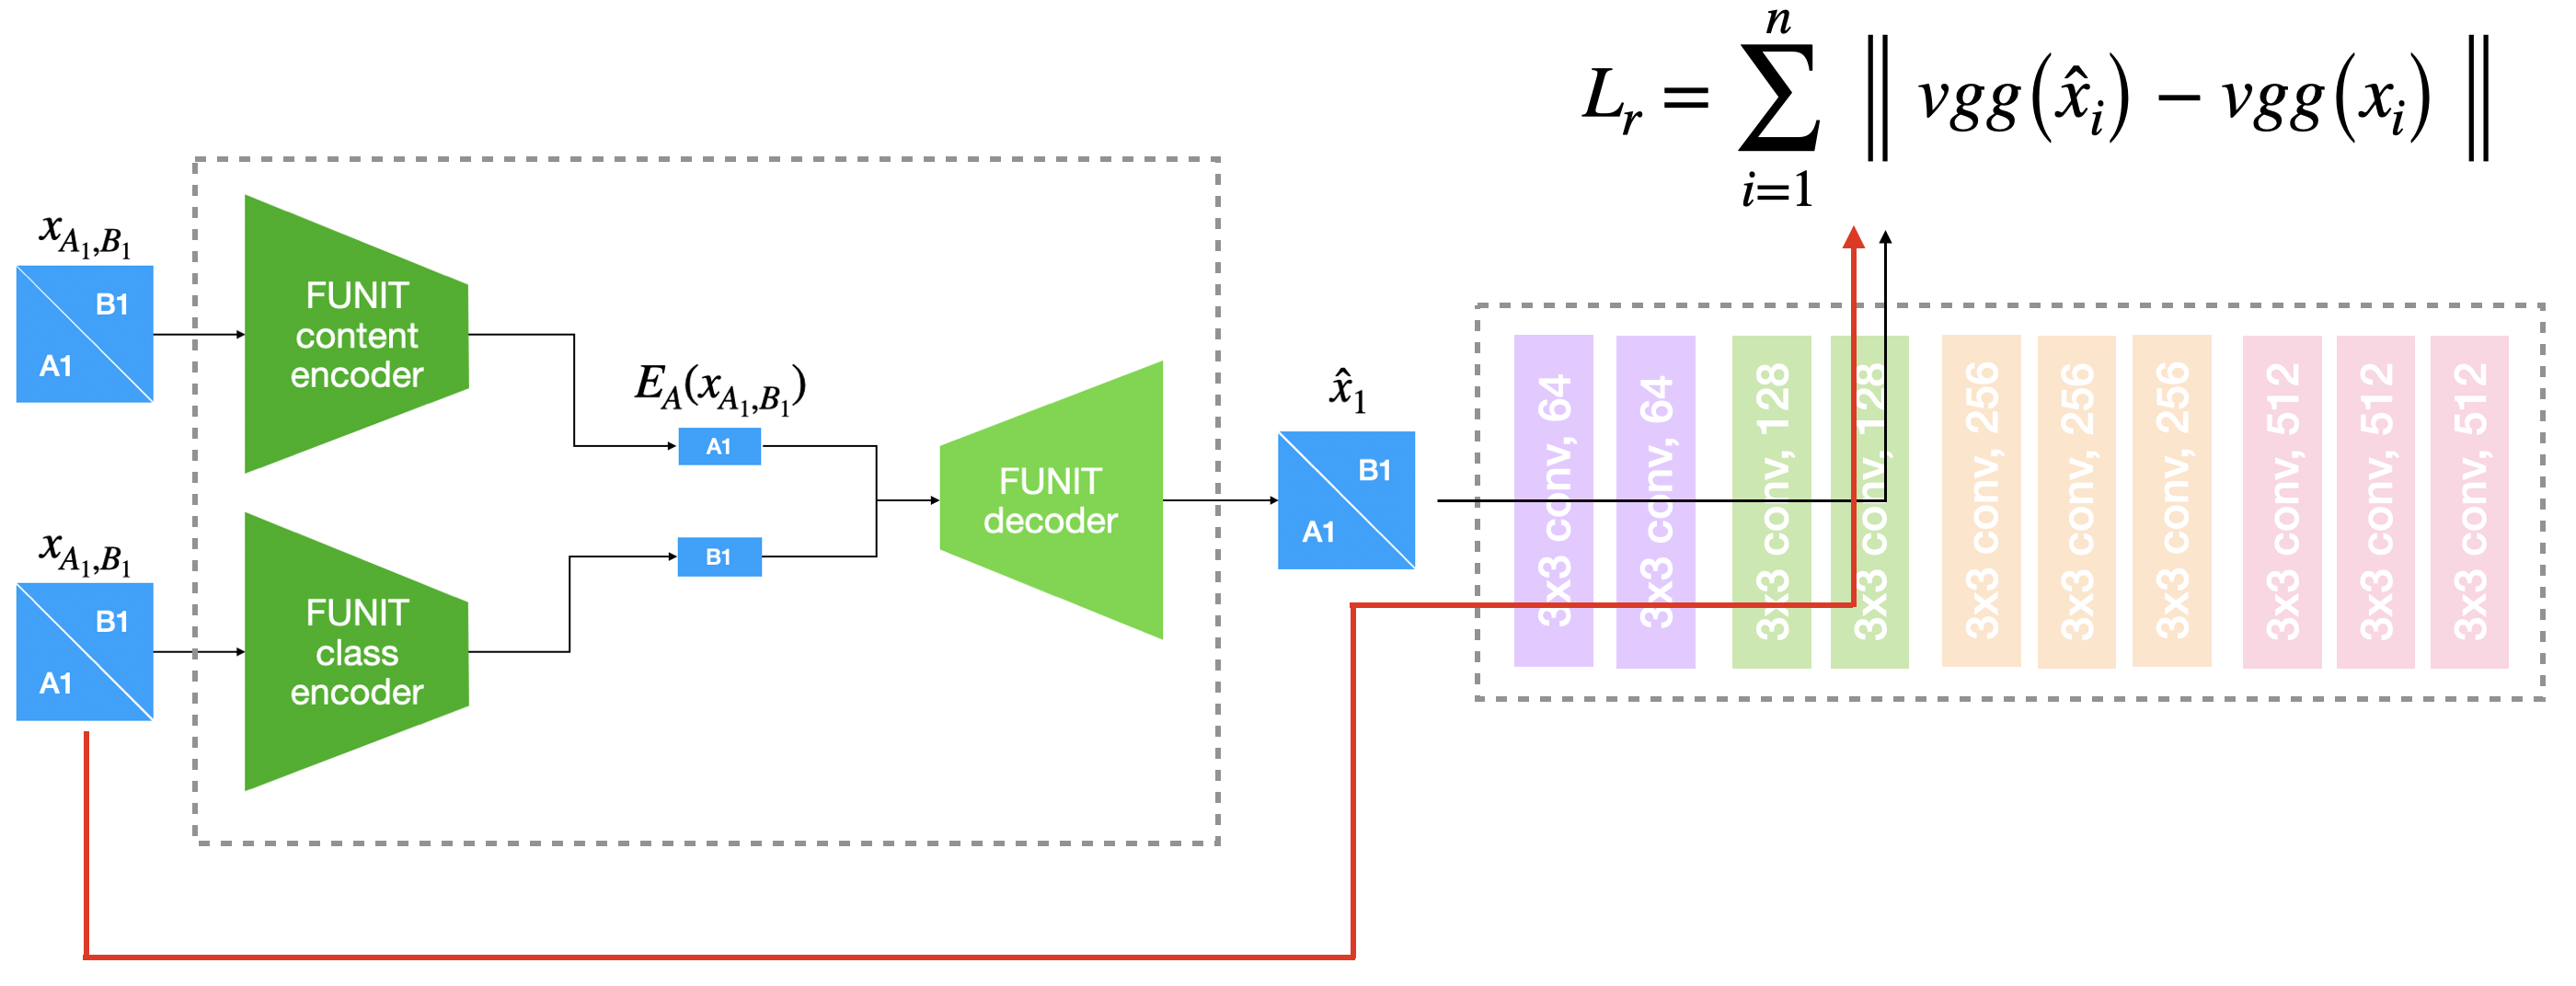
\includegraphics[width=1.0\linewidth]{figures/vgg_loss.png}
	\caption{VGG perceptual loss using pre-trained VGG16}
	\label{fig:vgg_loss}
\end{figure}

\paragraph{Next Steps}
\newline
We agreed on the following next steps via E-Mail:

\begin{description}
   \item[Step 1: Reconstruction using FUNIT Encoders + Decoder] \hfill \\
    We take the encoder and decoder architecture from FUNIT \cite{liu2019few} and train it only with a reconstruction loss to try to do a simple reconstruction. This means that we feed the same image into the network's class and content encoder and try to reconstruct it without mixing. As a loss function we use the VGG loss as Ron suggested. An overview can be seen in Figure \ref{fig:step1}, while the VGG loss is shown in Figure \ref{fig:vgg_loss} and is by Johnson et al. \cite{johnson2016perceptual}.
    \item[Step 2: Integrate FUNIT into G2G Architecture] \hfill \\
    If good visual results are obtained from the simple reconstruction we move on and integrate the FUNIT encoders and their decoder into our own architecture as shown in Figure \ref{fig:step2}. Here we add the cycle consistency losses on top of the VGG reconstruction loss of Step 1. Note that the loss is calculated over the original and reconstructed image, and not the original and mixed.
    \item[Step 3: Adjustment of GAN Discriminator and Loss] \hfill \\
    To increase photorealism and visual quality of the mixed images, we want to integrate adversarial training by comparing FUNIT's GAN loss to CycleGAN's loss.
\end{description}

\begin{multicols}{2}

\section{Notation}

To recall our notation: 

\begin{itemize}
	\item Original images \\$x_1 = x_{A_1,B_1}$ and $x_2 = x_{A_2,B_2}$
	\item Mixed images \\$\hat{x}_{A_1,B_2} = G \big (E_A(x_1), E_B(x_2) \big)$ and \\$\hat{x}_{A_2,B_1} = G \big (E_A(x_2), E_B(x_1) \big)$
	\item Reconstructed images \\$\hat{x}_1= G \big (E_A(\hat{x}_{A_1,B_2}), E_B(\hat{x}_{A_2,B_1}) \big)  $ and \\$\hat{x}_2  = G \big (E_A(\hat{x}_{A_2,B_1}), E_B(\hat{x}_{A_1,B_2}) \big)  $
\end{itemize}


\section{Simple Reconstruction using FUNIT}

\subsection{Architecture}

\textbf{Content Encoder} - We adopt the class and content encoder architecture of FUNIT. The content encoder encodes the separate feature while the class encoder encodes the "rest of the image". The content encoder consists of 4 [Conv, InstanceNorm, ReLU] layers followed by two ResBlocks while the first layer does not downsample the height and width, and the following three do downsample by half of their size. Note that $nfe$ stands for the number of feature maps and is 64. It takes a $3 \times 128 \times 128$ image as an input and produces a latent content code of size 5$12 \times 16 \times 16$, compare Figure \ref{fig:content_encoder}.\\
\newline
\textbf{Class Encoder} - The class encoder is made from 5 [Conv, InstanceNorm, ReLU] Layers and is followed by AvgPooling. The first layer does not downsample the height and width similarly to the content encoder, while the following four layers do. The AvgPooling layer also downsamples the height and width again by half of their size resulting in a latent class code of dimension $1024 \times 1 \times 1$, compare Figure \ref{fig:class_encoder}. Again, $nfe = 64$. The class code is more lightweight as it is fed into the decoder via AdaIN layers later.

\begin{Figure}
	\centering 
	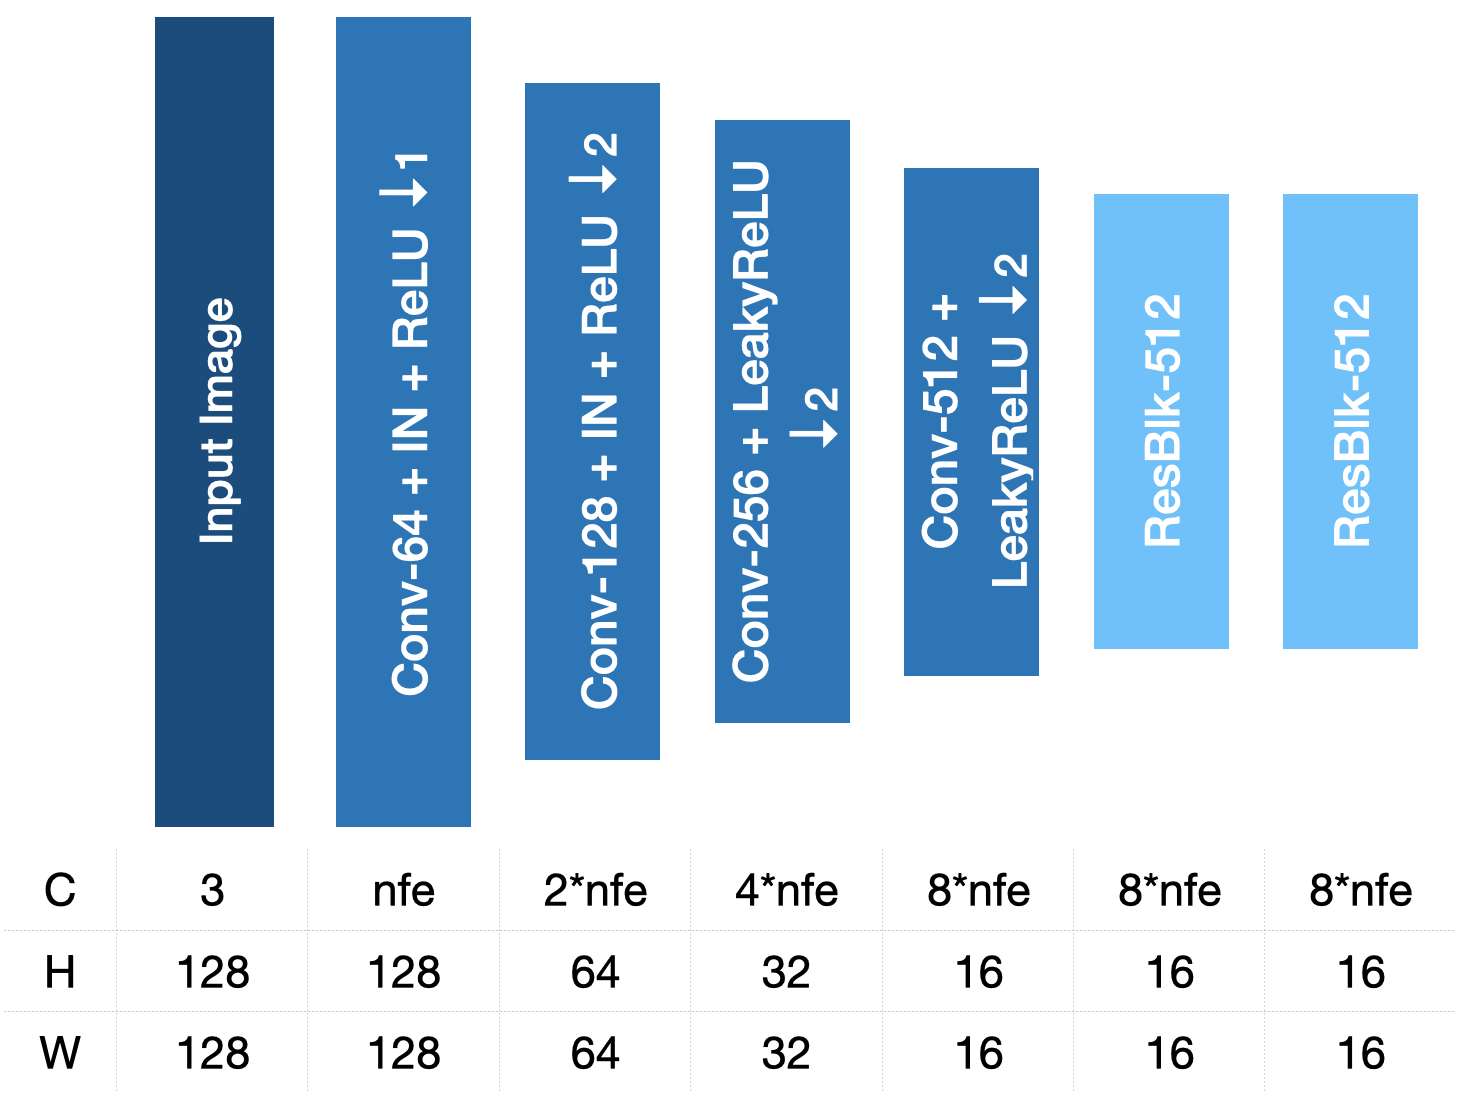
\includegraphics[width=\linewidth]{figures/content_encoder.png}
	\captionof{figure}{Content Encoder of FUNIT}
	\label{fig:content_encoder}
\end{Figure}


\begin{Figure}
	\centering 
	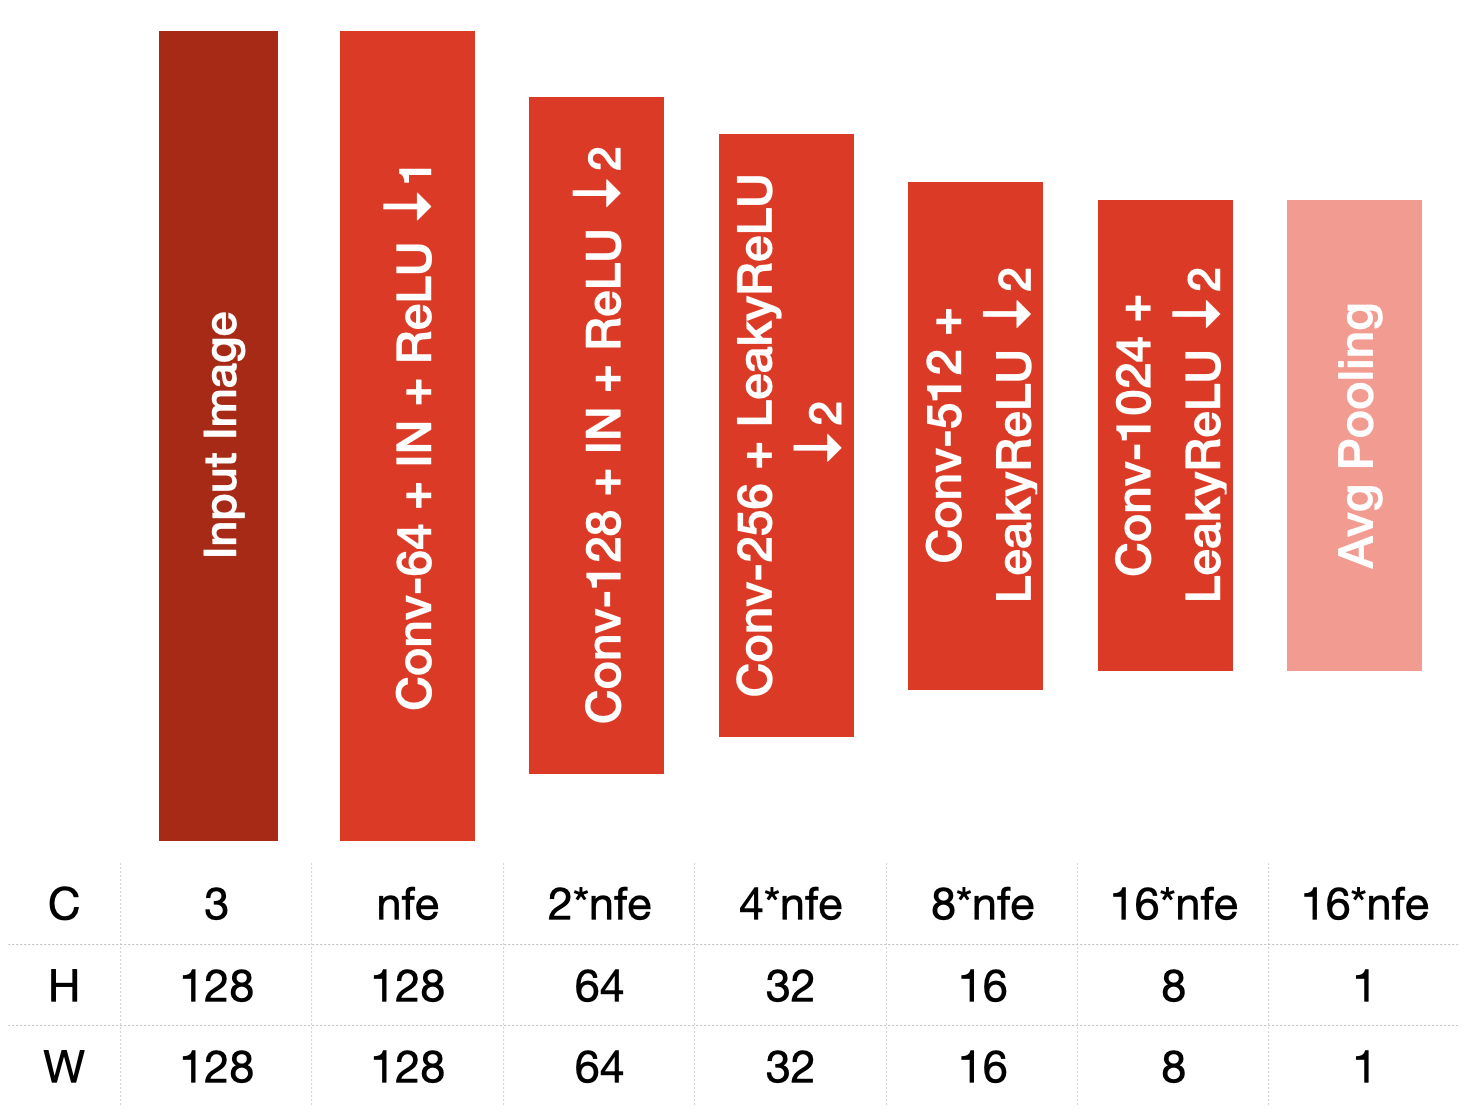
\includegraphics[width=\linewidth]{figures/class_encoder.png}
	\captionof{figure}{Class Encoder of FUNIT}
	\label{fig:class_encoder}
\end{Figure}

\paragraph{}

\textbf{Decoder} - The decoder takes to latent codes. The content code is taken directly as an input into the network, while the class code is fed through three fully connected layers, and then via AdaIn layers into the first two ResBlocks of the decoder. These ResBlocks are then followed by 3 [Conv, InstanceNorm, ReLU] layers which upsample the feature map dimensions by two. The final [Conv, tanh] layer then constructs the output image of the original dimension $3 \times 128 \times 128$, see Figure \ref{fig:decoder}.

\subsection{Losses}
In this very first step we use only the VGG perceptual loss by using a pre-trained VGG16 model. The input image and the reconstructed image are both fed into the VGG and the activations at the same layer are compared using mean squared error.
We chose the activations of relu layer 2\_2 to compare the features, see Figure \ref{fig:vgg_loss} and Equation \ref{eq:vgg}.

\begin{equation}
	L_{rec} = \sum_{i=1}^{n} \left\| vgg \big( \hat{x}_i \big)^{relu2\_2} - vgg \big( {x}_i \big)^{relu2\_2} \right\| 
	\label{eq:vgg}
\end{equation}

\subsection{Results}

Figure \ref{fig:results1} shows the visual result after training for only 2 epochs. The reconstructed image looks for human observers nearly the same aside from lighting differences.

\section{Integrate FUNIT into G2G Architecture}

As the first results have high visual quality we moved onto the next step, which is integrating the FUNIT encoders and their decoder into our G2G architecture as seen in Figure \ref{fig:step2}.

\subsection{Architecture and Implementation Details}

We take replace our original encoder $E_A$ and $E_B$ by FUNIT's content and class encoder, our generator has the architecture of FUNIT's decoder. Then, two different images are fed into the encoders respectively and mixed, the mixed images are again fed into the encoders and reconstructed as seen in Figure \ref{fig:step2}.

\subsection{Losses}

We adapt the VGG perceptual loss to fit our G2G architecture, this means that we feed the vgg with the original image $x_1$ and the reconstructed one $\hat{x_1}$. Also, we now add the cycle consistency losses \ref{eq:cyc1} and \ref{eq:cyc2}, shown below. These are the cycle consistency losses that we used before in our naive approach, but now with FUNIT architecture.

\begin{multline}
	L_{cyc,E_A} = \sum_{i=1}^{n-1} \left\| E_A(x_{A_i,B_i})- E_A(\hat{x}_{A_i,B_{i+1}})\right\| ^2+ 
	\\
	\left\| E_A(x_{A_{i+1},B_{i+1}}) - E_A(\hat{x}_{A_{i+1},B_i})\right\|^2
	\label{eq:cyc1}
\end{multline}
\begin{multline}
	L_{cyc,E_B} = \sum_{i=1}^{n-1} \left\| E_B(x_{A_i,B_i}) - E_B(\hat{x}_{A_{i+1},B_i})\right\| ^2+ 
	\\
	\left\| E_B(x_{A_{i+1},B_{i+1}}) - E_B(\hat{x}_{A_1,B_{i+1}})\right\|^2
	\label{eq:cyc2}
\end{multline}
\begin{multline}
	L = L_{rec} + \gamma \cdot (L_{cyc,E_A} + L_{cyc,E_B})
	\label{eq:all}
\end{multline}

\subsection{Results}

For the results of this second step we used the plot with the same layout as last time, i.e. the top row shows the images $x_1$ and $x_2$, the second row, the mixed images and the last row the reconstructed images $\hat{x_1}$ and $\hat{x_2}$. The visual results can be seen in Figure \ref{fig:gam_0.4} for $\gamma = 0.01$. The grid search is currently still running, so we are expecting more results for $\gamma = 0.4$, $\gamma = 1.3$, $\gamma = 10$ and $\gamma = 100$.

\begin{Figure}
	\centering 
	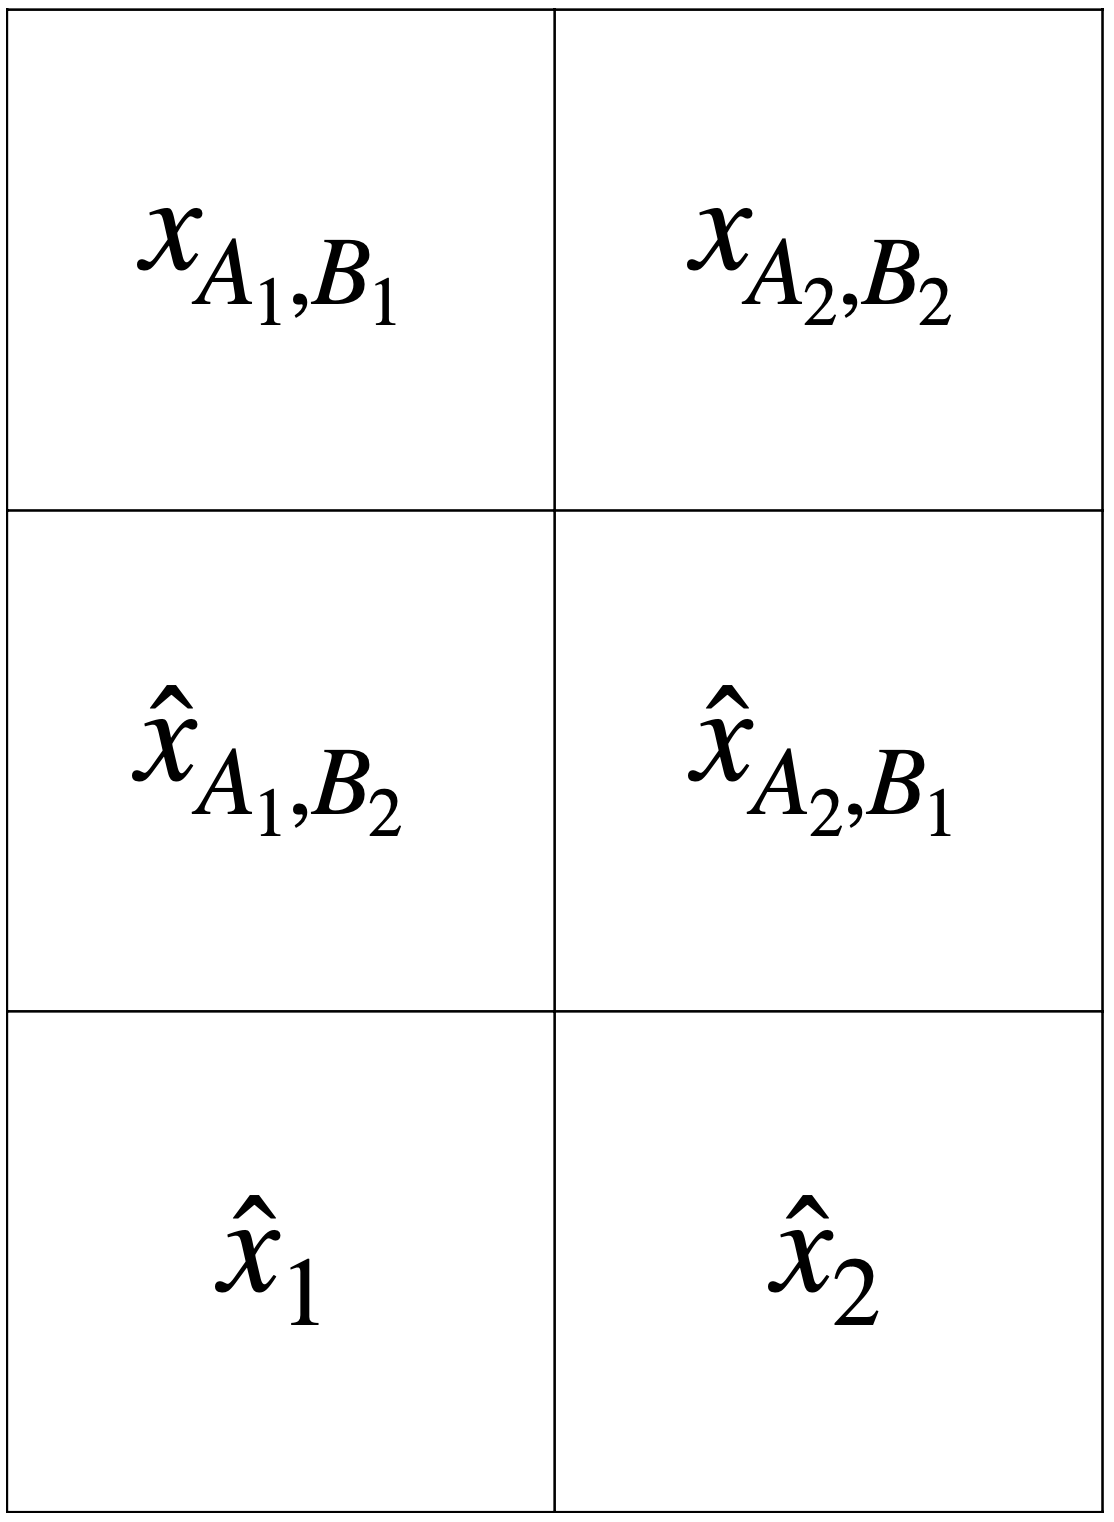
\includegraphics[width=0.7\linewidth]{figures/layout.png}
	\captionof{figure}{Layout for Plots}
	\label{fig:layout}
\end{Figure}

\section{Future Work}
\textbf{Next Steps}
\begin{enumerate}
	\item Evaluate the upcoming results from different $\gamma$ values. As suggested by Ron, we also include extreme gamma values, such as 0.01, 10 and 100.
	\item Implement GAN Loss using FUNIT and CycleGAN architecture and loss
\end{enumerate}

\noindent \textbf{Open Questions}
\begin{enumerate}
	\item The quality of the mixed images degraded during the epochs. We assume that due to the currently small weight of 0.01 on the cycle consistency losses, the reconstruction loss gets much stronger and minimizes its loss at the expense of the cycle consistency loss. We have fixed the VGG reconstruction loss weight at 1.0. We assume that tuning the $\gamma$ hyperparameter as well as introducing the GAN loss would improve this visual quality.
	\item Until the current state of the grid search, i.e. $\gamma = 0.01$ we don't see any disentanglement yet. Is this due to the setting of the hyperparameter or are there any other possible reasons why disentanglement does not yet work?
	\item Would it be a good idea to use FUNIT's loss instead of the VGG perceptual loss? That is:
    \begin{equation}
    	L_{recon} = \frac{1}{n} \sum_{i=1}^{n} \left\| predict - target \right\| 
    	\label{eq:funit}
    \end{equation}
	\item Where do the shiny highlights in the mixed images come from? They do not seem to always minimize the reconstruction (at least visually), since they are not always located where the light hits the face or head but are located where there's background.
\end{enumerate}

\end{multicols}

% RESULTS
\begin{figure}[h!]
	\centering 
	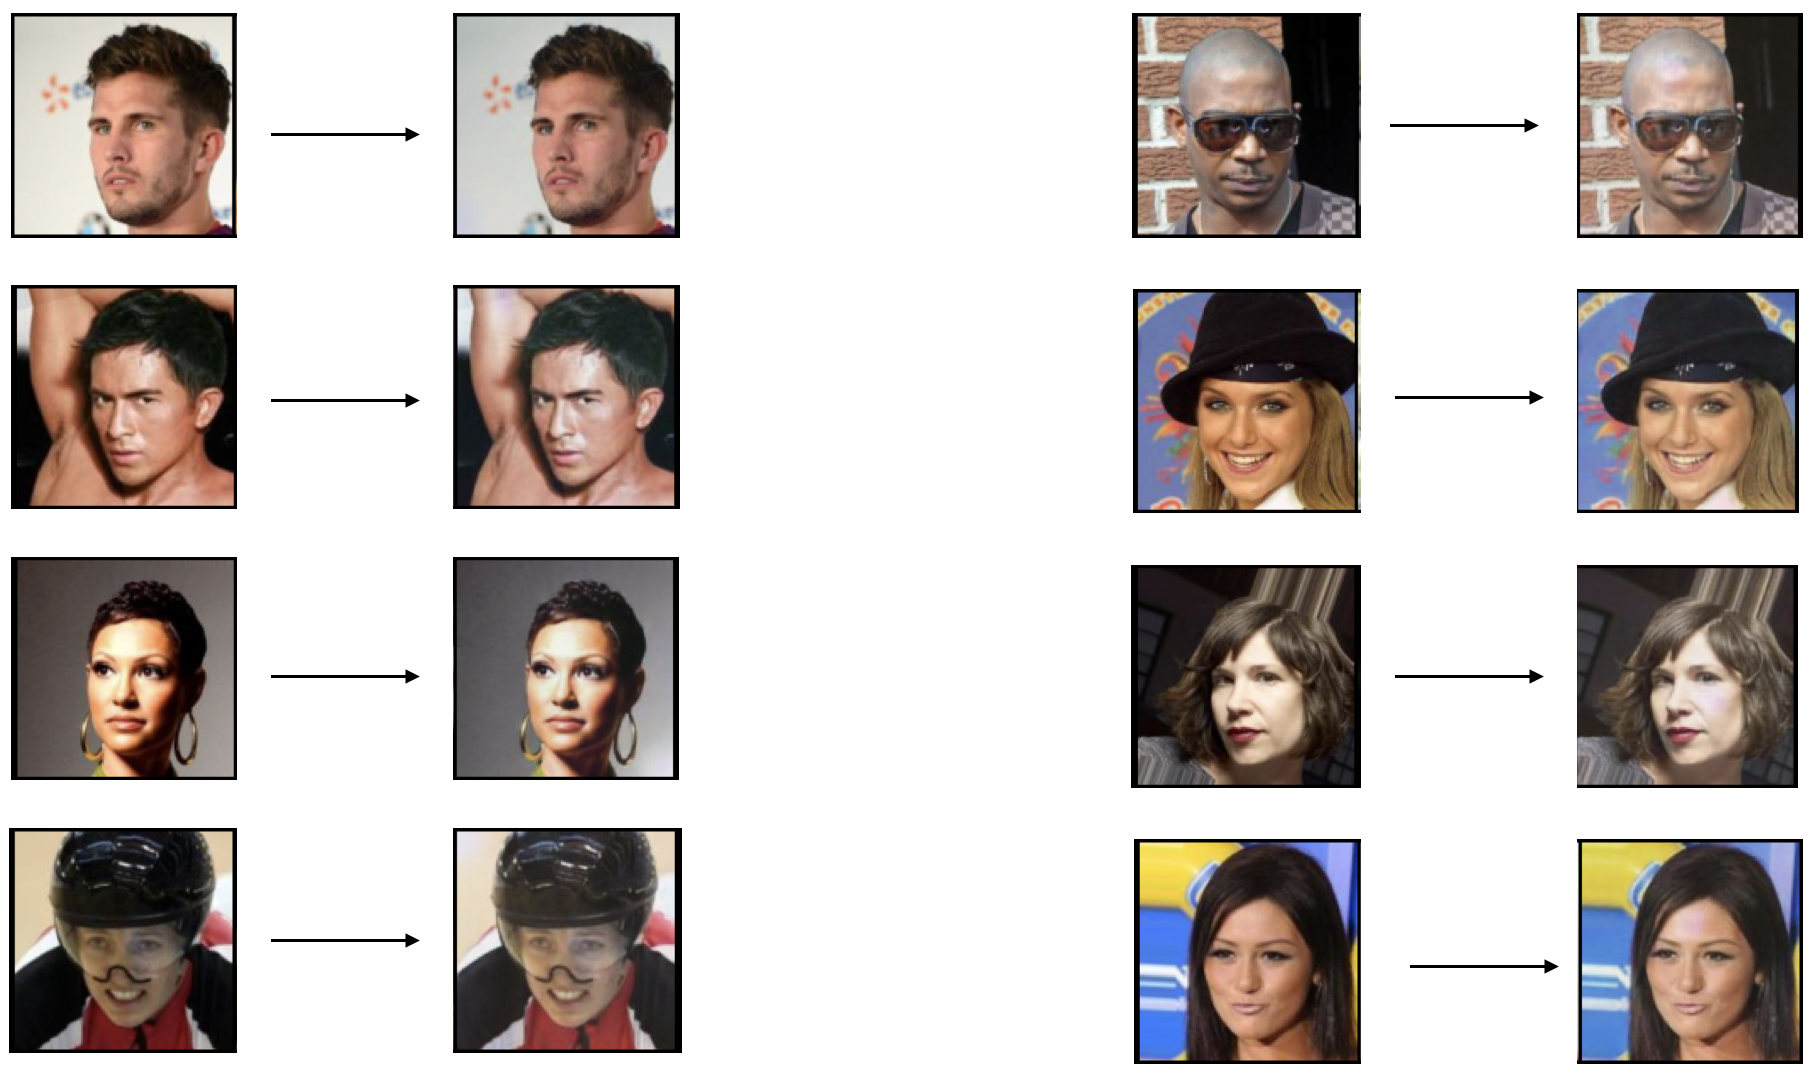
\includegraphics[width=\linewidth]{{figures/results1}.png}
	\caption{Plots from validation set for Step 1}
	\label{fig:results1}
\end{figure}
\begin{figure}[h!]
	\centering 
	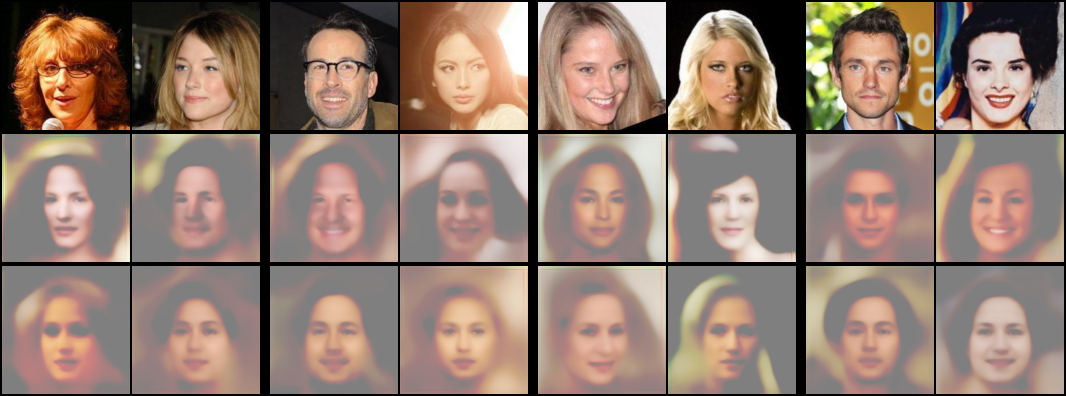
\includegraphics[width=0.8\linewidth]{{figures/gam_0.01}.png}
	\caption{Plots from validation set with $\gamma = 0.01$}
	\label{fig:gam_0.4}
\end{figure}

\FloatBarrier
\printbibliography

\end{document}